\documentclass[11pt]{article}
\usepackage{amsmath, amssymb, amsfonts,  graphicx, enumerate, float, wrapfig, hyperref}
\usepackage[margin=0.5in]{geometry}
\graphicspath{{./}}
\newcommand*{\vs}{\vspace{1cm}}
\newcommand*{\next}{\noindent}
\newcommand*{\set}{\setcounter{equation}{0}}

\begin{document}

\title{Notes - 4.2 Area}
\author{Juan J. Moreno Santos}
\date{November 2023}

\maketitle

\section{Warm-up 11/14/2023}
1. If $x+7y=29$ is an equation of the line normal (perpendicular) to the graph of f(x) at the point (1, 4), then $f'(x)=$\\
Find the slope of the line by putting the equation in slope-intercept form:
\begin{align}
    7y=-x+29\\
    y=-\frac{1}{7}+b
\end{align}
We don't consider b in this problem.\\
Now, the reciprocal of $-\frac{1}{7}$ is
\begin{align}
    7
\end{align}
Therefore, $f'(x)=7$.

\vs
\next
Find $\frac{d}{dx}(y^2-2xy=16)$ by implicit differentiation:
\begin{align}
    \set
    2ydy-(xdy+ydx)&=0\\
    2ydy-2xdy&=2ydx\\
    (2y-2x)dy&=2ydx\\
    \frac{dy}{dx}&=\frac{2y}{2y-2x}\\
    &=\frac{2y}{2(y-x)}\\
    &=\frac{y}{y-x}
\end{align}

\section{4.2 Area}
\begin{enumerate}
    \item Use sigma notation (summation) to write and evaluate a summation
    \item Understand the concept of Area
    \item Approximate the area of a plane region
    \item Find the area of a plane region using limits
\end{enumerate}

\subsection{Sigma notation}
The sum of $n$ terms $a_1, a_2, a_3,\cdots a_n$ is written as
\[\sum_{i=1}^{n}a_i=a_1+a_2+a_3+\cdots+a_n\]
Where 
\begin{enumerate}
    \item $i$ is the index of summation
    \item $a_i$ is the $i$th term of the sum
    \item $n$ and $1$ are the upper and lower bounds of summation, respectively
\end{enumerate}

\subsection{Examples of Sigma Notation}
\begin{align}
    \set
    \sum_{i=1}^{6}&i=1+2+3+4+5+6\\
    \sum_{i=0}^{5}&(i+1)=1+2+3+4+5+6\\
    \sum_{j=3}^{7}&j^2=3^2+4^2+5^2+6^2+7^2\\
    \sum_{k=1}^{n}&\frac{1}{n}(k^2+1)=\frac{1}{n}(1^2+1)+\frac{1}{n}(2^2+1)+\cdots+\frac{1}{n}(n^2+1)\\
    \sum_{i=1}^{n}&f(x_i)\Delta x=f(x_1)\Delta x+f(x_2)\Delta x+\cdots+f(x_n)\Delta x
\end{align}
Notice how (a) and (b) are the same sequence, but notated differently.

\subsection{Approximating the area under a function using summation}
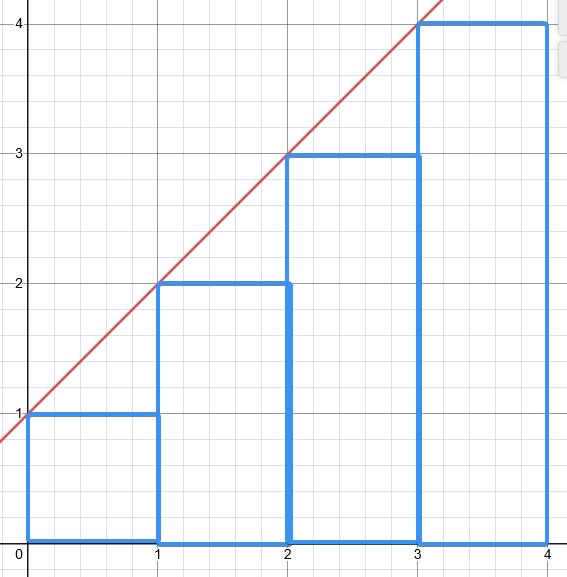
\includegraphics{xplus1.png}\\
Consider that $n=4$ and $f$ is in the [0, 4] interval. The sum of the rectangles without sigma notation is written as:
\[h_1\cdot b+h_2+\cdot b+ h_3\cdot b+h_4\cdot b\]
Which is the same as:
\[f(x_1)b+f(x_2)b+f(x_3)b+f(x4)b\]
The iterations of $x$ represent $\Delta x$
In Sigma Notation, this is written as:
\[\sum_{i=1}^{n}f(x_1)\Delta x=\sum_{i=0}^{3}(i+1)1=10\]
\subsection{Properties of summation}
\begin{align}
    \set
    \sum_{i=1}^{n}&ka_i=k\sum_{i=1}^{n}a_i\\
    \sum_{i=1}^{n}&(a_i\pm b_i)=\sum_{i=1}^{n}a_i\pm\sum_{i=1}^{n}b_i\\
\end{align}
Considering that
\[\Delta x=\frac{b-a}{n}=\frac{4-0}{n}=\frac{4}{n}\]
and
\[x_i=\frac{4}{n}i\]
Therefore,
\begin{align}
    \set
    \lim_{n\to\infty}\sum_{i=0}^{n}&(i+1)\Delta x=\lim_{\Delta x\to 0}\sum_{i=0}^{n}(i+1)\Delta x\\
    \lim_{n\to\infty}\sum_{i=0}^{n}&(i+1)\Delta x=\Delta x(\sum x_i+\sum 1)\\
    &=\frac{4}{n}(\sum \frac{4i}{n}+\sum 1)\\
    &=\frac{4}{n}\left(\frac{4}{n}\left(\frac{n(n+1)}{2}\right)+n\right)\\
    &=\frac{4}{n}\left(\frac{4n(n+1)}{2n}+\frac{n2n}{2n}\right)\\
    &=\frac{4}{n}\left(\frac{4n^2+4n+2n^2}{2n}\right)
\end{align}
Taking the limit,
\begin{align}
    \set
    \lim_{h\to\infty}\frac{24n^2+16n}{2n^2}
    =12
\end{align}
\subsection{Summation formulas}
\begin{align}
    \set
    \sum_{i=1}^{n}&c=cn\\
    \sum_{i=1}^{n}&i=\frac{n(n+1)}{2}\\
    \sum_{i=1}^{n}&i^2=\frac{n(n+1)(2n+1)}{6}\\
    \sum_{i=1}^{n}&i^3=\frac{n^2(n+1)^2}{4}
\end{align}

\subsection{Example - Evaluating a sum}
Evaluate $\sum_{i=1}^{n}\frac{i+1}{n}$ for $n=10$, 100, 1000, and 10000.
\begin{align}
    \set
    \sum_{i=1}^{n}\frac{i+1}{n^2}&=\frac{1}{n^2}\sum_{i=1}^{n}(i+1)\\
    &=\frac{1}{n^2}\left(\sum_{i=1}^{n}i+\sum_{i=1}^{n}1\right)\\
    &=\frac{1}{n^2}\left(\frac{n(n+1)}{2}+n\right)\\
    &=\frac{1}{n^2}\left(\frac{n^2+3n}{2}\right)\\
    &=\frac{n+3}{2n}
\end{align}
Steps:
\begin{enumerate}[(a)]
    \item Factor $\frac{1}{n^2}$ out of the sum.
    \item Write as two sum
    \item Apply summation formulas 1 and 2
    \item Simplify the expression
\end{enumerate}

Taking the limit:\\
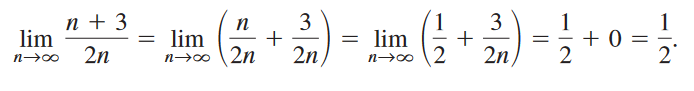
\includegraphics{limit.png}

\section{Warm-up 11/16/2023}
1. If $f(x)=x\sqrt[]{x}$ then $f'(1)=$
\begin{align}
    \set
    &\frac{d}{dx}(x\sqrt[]{x})\\
    &=\frac{d}{dx}(x\cdot x^{1/2}=x^{3/2})\\
    &=\frac{3}{2}x^{1/2}\\
    f'(1)&=\frac{3}{2}(1)^{1/2}=\frac{3}{2}
\end{align}
2. If the line y=3x-5 is tangent to the graph of $y=f(x)$ at the point (4, 7) then $\lim{x\to 0}\frac{f(4+x)-f(4)}{x}$ is:\\
\indent Remember that this expression is the exact limit definition of the derivative at a certain point (h is changed to x in this case). The slope of the tangent line is 3 because the equation is in the form $y=mx+b$. 

\section{Limits of the lower and upper sums}
Let $f$ be continouous and nonnegative on the interval [a, b]. The limits as $n\to\infty$ of both the lower and upper sums exist and are equal to each other. That is,
\begin{align}
    \set
    \lim_{n\to\infty}s(n)&=\lim_{n\to\infty}\sum_{i=1}^{n}f(m_i)\Delta x\\
    &=\lim_{n\to\infty}\sum_{i=1}^{n}f(M_i)\Delta x\\
    &=\lim_{n\to\infty}S(n)
\end{align}
where $\Delta x=\frac{b-a}{n}$ and $f(m_i)$ and $f(M_i)$ are the minimum and maximum values of $f$ on the subinterval.

\section{Definition of the are of a region in the plane}
Let $f$ be continuous and nonnegative on the interval [a, b]. The are of the region bounded by the graph of $f$, the x-axis, and the vertical lines $x=a$ and $x=b$ is
\[\text{Area}=\lim_{n\to\infty}\sum_{i=1}^{n}f(x_i)\Delta x=\int_{a}^{b}f(x)dx\]
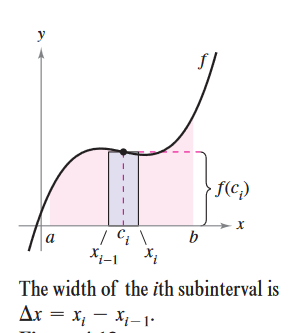
\includegraphics{area.png}

\section{The fundamental theorem of Calculus}
Remember that
\begin{align}
    \set
    \frac{d}{dx}(F)&=f\\
    \frac{d}{dx}(f)&=f'
\end{align}
Therefore,
\[\int_{a}^{b}f(x)dx=F(b)-f(a)\]
\subsection{Applying the fundamental theorem of Calculus}
1. Consider the previous function $f(x)=x+1$. By that, $F(x)=\frac{1}{2}x^2$
\begin{align}
    \set
    &\int_{0}^{4}x+1dx\\
    &=\frac{1}{2}x^2+x+C|_{0}^{4}\\
    &=\frac{1}{4}^2+(4)+C-(\frac{1}{2}(0)^2+0+C)\\
    &=12u^2
\end{align}

\vs
\next
2. \begin{align}
    \set
    &\int_{0}^{\pi}\sin xdx\\
    &=-\cos x|_{0}^{\pi}\\
    &=-(-1)-(-1)\\
    &=2
\end{align}

\section{P-set 76}
Use the Midpoint Rule
\[\text{Area}\approx \sum_{i=1}^{n}f\left(\frac{x_1+x_{i-1}}{2}\right)\Delta x\]
with $n=4$ to approximate the are of the region bounded by the graph of the function and the x-axis over the given interval
\[f(x)=\sin x,\,\,\,\,\left[0,\,\,\frac{\pi}{2}\right],\,\,\,\, n=4\]
Let \[c_i=\frac{x_i+x_i-1}{2}\]
\begin{align}
    \set
    \Delta x&=\frac{\pi}{8},\,\,\,\, c_1=\frac{\pi}{16},\,\,\,\, c_2=\frac{3\pi}{16},\,\,\,\, c_3=\frac{5\pi}{16},\,\,\,\ c_4=\frac{7\pi}{16}\\
    \text{Area}&\approx \sum_{i=1}^{n}f(c_1)\Delta x=\sum_{i=1}^{4}\sin\left(\frac{(2n-1)\pi}{16}\right)\frac{\pi}{8}\\
    &\approx 1.006
\end{align}
\section{Solving differential equations}
\subsection{Separate}
\begin{align}
    \set
    \frac{dy}{dx}&=12x^3\\
    dy&=12x^3dx
\end{align}
\subsection{Integrate}
\begin{align}
    \set
    \int dy&=\int 12x^3dx\\
    y+C_1&=3x^4+C_2\\
    y&=3x^4+C_3
\end{align}





\end{document}